\section{Metal reflectance of silver and gold}

This example uses experimental optical constants instead of fabricated
values. The refractive index of silver and gold is taken from the
Johnson--Christy tabulation sampled
at the ten wavelengths \SI{400}{}, \SI{450}{}, \SI{500}{}, \SI{550}{},
\SI{600}{}, \SI{650}{}, \SI{700}{}, \SI{800}{}, \SI{900}{},
\SI{1000}{\nano\metre}, and linearly interpolated on a 601-point grid
between $\SI{400}{}$ and $\SI{1000}{\nano\metre}$. The stack is reduced to
two half-spaces, air against metal, and the reflectance is evaluated at
normal incidence for both materials.

For a bare interface the $s$- and $p$-polarisations coincide, and the
normal-incidence reflectance follows directly from the Fresnel
coefficients as
\begin{equation}
  R = \frac{(n - 1)^{2} + k^{2}}{(n + 1)^{2} + k^{2}}, \label{eq:metal-R}
\end{equation}
with $N = n + \ii k$ the complex refractive index at the given wavelength.
Equation~\eqref{eq:metal-R} is the strong reference against which the TMM
result is compared: any disagreement would indicate an error in the
branch-cut choice for complex $N$ or in the evaluation of the
single-interface Fresnel coefficient at $\theta_0 = 0$.

\begin{center}
\begin{tikzpicture}
  \fill[black!4]   (0, 0) rectangle (5, 1.6);
  \fill[yellow!35] (0,-1.2) rectangle (5, 0);
  \draw[thick] (0,0) -- (5,0);
  \node[lbl, anchor=east] at (4.9, 1.2) {air};
  \node[lbl, anchor=east] at (4.9,-0.7) {Ag or Au};
  \raysketch{1.6}{0}{f}
\end{tikzpicture}
\end{center}

\begin{figure}[!htbp]
  \centering
  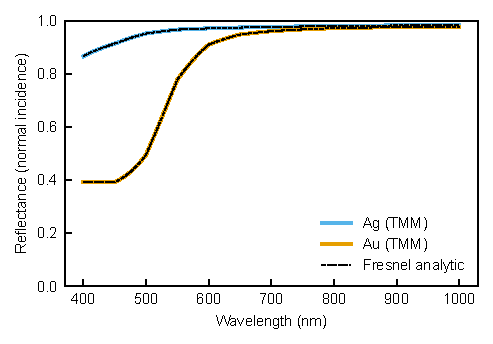
\includegraphics[width=0.5\textwidth]{09_metal_reflectance.pdf}
  \caption{Reflectance of bulk silver and bulk gold from \SIrange{400}{1000}{\nano\metre} at normal incidence. TMM (solid) is overlaid on the closed-form Fresnel expression~\eqref{eq:metal-R} evaluated from the same tabulated $N(\lambda)$.}
  \label{fig:metal}
\end{figure}

The TMM reproduces~\eqref{eq:metal-R} at
$\max|\Delta R| \approx \num{1e-15}$ for silver and $\num{9e-16}$ for
gold. Silver remains above $R \approx 0.95$ across the whole visible and
near-infrared range; gold shows the characteristic absorption edge that
pulls the reflectance down below \SI{500}{\nano\metre}, with the
reflectance rising again and saturating near unity in the red and
near-infrared. The identity of the two curves to floating-point precision
confirms that tabulated complex indices are ingested and propagated
consistently by the code.


